%\documentclass{beamer} % descomentar para tener pausas
\documentclass[handout]{beamer} % descomentar para no tener pausas
\usetheme{CambridgeUS}
%\setbeamertemplate{background}[grid][step=8 ] % cuadriculado

\usepackage[utf8]{inputenc}%esto permite (en Windows) escribir directamente 
\usepackage{graphicx}
\usepackage{array}
\usepackage{tikz} 
\usetikzlibrary{shapes,arrows,babel,decorations.pathreplacing}
\usepackage{verbatim} 
\usepackage{xcolor} 
\usepackage{amsgen,amsmath,amstext,amsbsy,amsopn,amsfonts,amssymb}
\usepackage{amsthm}
\usepackage{tikz}
\usepackage{tkz-graph}
\usepackage{mathtools}
\usepackage{xcolor}

%\setbeamertemplate{background}[grid][step=8 ]
\setbeamertemplate{itemize item}{$\circ$}
\setbeamertemplate{enumerate items}[default]

\definecolor{links}{HTML}{2A1B81}
\hypersetup{colorlinks,linkcolor=,urlcolor=links}

\newcommand{\img}{\operatorname{Im}}
\newcommand{\nuc}{\operatorname{Nu}}
\newcommand\im{\operatorname{Im}}
\renewcommand\nu{\operatorname{Nu}}
\newcommand{\la}{\langle}
\newcommand{\ra}{\rangle}
\renewcommand{\t}{{\operatorname{t}}}
\renewcommand{\sin}{{\,\operatorname{sen}}}
\newcommand{\Q}{\mathbb Q}
\newcommand{\R}{\mathbb R}
\newcommand{\C}{\mathbb C}
\newcommand{\K}{\mathbb K}
\newcommand{\F}{\mathbb F}
\newcommand{\Z}{\mathbb Z}

\renewcommand{\figurename }{Figura}
%\usepackage{enumitem}
%\setlist[itemize]{itemsep=10pt, label={$\circ$}}
%\newtheorem{teorema}{Teorema}
%\newtheorem{corolario}[teorema]{Corolario}
%\newtheorem{proposicion}[teorema]{Proposición}

%\theoremstyle{definition}
%\newtheorem{definicion}[theorem]{Definici\'on}
%\newtheorem{ejemplo}[theorem]{Ejemplo}
%\newtheorem{pregunta}[equation]{Pregunta}
%\newtheorem{step}{Paso}



\newenvironment{exercise}[1]% environment name
{% begin code
    \par\vspace{\baselineskip}\noindent
    \textbf{Ejercicio (#1)}\begin{itshape}%
        \par\vspace{\baselineskip}\noindent\ignorespaces
    }%
    {% end code
    \end{itshape}\ignorespacesafterend
}


\newenvironment{definicion}% environment name
{% begin code
    \par\vskip .2cm%
    {\color{blue}Definición}%
    \vskip .2cm
}%
{%
    \vskip .2cm}% end code

\newenvironment{observacion}% environment name
{% begin code
    \par\vskip .2cm%
    {\color{blue}Observación}%
    \vskip .2cm
}%
{%
    \vskip .2cm}% end code

\newenvironment{ejemplo}% environment name
{% begin code
    \par\vskip .2cm%
    {\color{blue}Ejemplo}%
    \vskip .2cm
}%
{%
    \vskip .2cm}% end code

\newenvironment{ejercicio}% environment name
{% begin code
    \par\vskip .2cm%
    {\color{blue}Ejercicio}%
    \vskip .2cm
}%
{%
    \vskip .2cm}% end code


\renewenvironment{proof}% environment name
{% begin code
    \par\vskip .2cm%
    {\color{blue}Demostración}%
    \vskip .2cm
}%
{%
    \vskip .2cm}% end code



\newenvironment{demostracion}% environment name
{% begin code
    \par\vskip .2cm%
    {\color{blue}Demostración}%
    \vskip .2cm
}%
{%
    \vskip .2cm}% end code

\newenvironment{idea}% environment name
{% begin code
    \par\vskip .2cm%
    {\color{blue}Idea de la demostración}%
    \vskip .2cm
}%
{%
    \vskip .2cm}% end code

\newenvironment{solucion}% environment name
{% begin code
    \par\vskip .2cm%
    {\color{blue}Solución}%
    \vskip .2cm
}%
{%
    \vskip .2cm}% end code



\newenvironment{lema}% environment name
{% begin code
    \par\vskip .2cm%
    {\color{blue}Lema}\begin{itshape}%
        \par\vskip .2cm
    }%
    {% end code
    \end{itshape}\vskip .2cm\ignorespacesafterend
}

\newenvironment{proposicion}% environment name
{% begin code
    \par\vskip .2cm%
    {\color{blue}Proposición}\begin{itshape}%
        \par\vskip .2cm
    }%
    {% end code
    \end{itshape}\vskip .2cm\ignorespacesafterend
}

\newenvironment{teorema}% environment name
{% begin code
    \par\vskip .2cm%
    {\color{blue}Teorema}\begin{itshape}%
        \par\vskip .2cm
    }%
    {% end code
    \end{itshape}\vskip .2cm\ignorespacesafterend
}


\newenvironment{corolario}% environment name
{% begin code
    \par\vskip .2cm%
    {\color{blue}Corolario}\begin{itshape}%
        \par\vskip .2cm
    }%
    {% end code
    \end{itshape}\vskip .2cm\ignorespacesafterend
}

\newenvironment{propiedad}% environment name
{% begin code
    \par\vskip .2cm%
    {\color{blue}Propiedad}\begin{itshape}%
        \par\vskip .2cm
    }%
    {% end code
    \end{itshape}\vskip .2cm\ignorespacesafterend
}

\newenvironment{conclusion}% environment name
{% begin code
    \par\vskip .2cm%
    {\color{blue}Conclusión}\begin{itshape}%
        \par\vskip .2cm
    }%
    {% end code
    \end{itshape}\vskip .2cm\ignorespacesafterend
}




\title[Clase 2 - Producto escalar y ortogonalidad]{Álgebra/Álgebra II \\ Clase 2 - Producto escalar y ortogonalidad en $\R^n$}
%\author[C. Olmos / A. Tiraboschi]{Carlos Olmos / Alejandro Tiraboschi}
\institute[]{\normalsize FAMAF / UNC
    \\[\baselineskip] ${}^{}$
    \\[\baselineskip]
}
\date[14/03/2024]{14 de marzo de 2024}




\begin{document}
    
    \frame{\titlepage} 

        
    \begin{frame}
        
        En este clase introduciremos la noción de ``producto escalar'' y posteriormente  ``norma'', ``distancia'' y ``ángulo'' en $\R^n$ usando el producto escalar.
        
        \
        
        Además veremos la noción de perpendicularidad u ortogonalidad.
        
        
        \
        
        Estas diapositivas están basadas en la Secciones 1.2 y  1.3 de las {\it Notas de Álgebra II} disponibles en Classroom. Allí se pueden encontrar más detalles y el sustento teórico de todas nuestras afirmaciones.
    \end{frame}
    
    
    
    
\begin{frame}\frametitle{Producto escalar}
            
    En 2-espacios, dados dos vectores $v = (x_1, x_2)$ y $w= (y_l, y_2)$, definimos su \textit{producto escalar}\index{producto escalar} como
    \begin{equation*}
    \langle v , w  \rangle :=x_1y_1 + x_2y_2.
    \end{equation*}\pause
    Para el caso de 3-espacios, sean   $v = (x_1, x_2,x_3)$ y $w= (y_l, y_2,y_3)$,  entonces el \textit{producto escalar de $v$ y $w$} es
    \begin{equation*}
    \langle v , w  \rangle :=x_1y_1 + x_2y_2+x_3y_3.
    \end{equation*}\pause
    Finalmente, en los $n$-espacios,  generalizamos la definición de la manera obvia: sean  $v = (x_1, \ldots,x_n)$ y $w= (y_l, \ldots,y_n)$,  definimos el \textit{producto escalar de $v$ y $w$} por        
    \begin{equation*}
    \langle v , w \rangle :=x_1y_1 + x_2y_2+\cdots+x_ny_n.
    \end{equation*}
\end{frame}



\begin{frame}
    Es importante notar  que este ``producto'' es un número real. 
    
    \vskip .4 cm \pause
    Por ejemplo, si
    \vskip .2 cm 
    \begin{equation*}
    v= (1, 3, - 2) \quad\text{ y } \quad w= (- 1, 4, - 3),
    \end{equation*}
    entonces
    \begin{equation*}
    \langle v , w \rangle= 1 \cdot(-1) +3\cdot 4 + (-2) \cdot (-3) = -1 + 12 + 6 = 17.
    \end{equation*}
    \vskip .2 cm \pause
    En  algunos libros de texto se denota al producto escalar como $v \cdot w$.
    \vskip .6 cm 
    Por el momento, no le damos una interpretación geométrica al producto escalar y veremos esto cuando veamos la norma de un vector. 
    \vskip 1 cm 
\end{frame}



\begin{frame}\frametitle{Propiedades básicas del producto escalar}
    
Las siguientes propiedades son  básicas y muy importantes. 
\vskip .3 cm \pause
Sean $v$, $w$, $u$  tres vectores, entonces

\vskip .3 cm \pause

\begin{enumerate}
    \item[\textbf{P1.}]    $\langle v , w \rangle = \langle w , v \rangle$.\pause
    \vskip .3 cm 
    \item[\textbf{P2.}] $\langle v , w + u \rangle =\langle v , w \rangle + \langle v , u \rangle$ y 
    \item[\,] $\langle v + w , u \rangle=\langle v , u \rangle + \langle w , u \rangle$.
    \vskip .3 cm \pause
    \item[\textbf{P3.}] Si $\lambda$ es un número, entonces 
    \begin{equation*}
    \langle \lambda v , w \rangle = \lambda \langle v , w \rangle \quad \text{ y } \quad  \langle v , \lambda w \rangle = \lambda \langle v , w \rangle.
    \end{equation*}
    \vskip .3 cm \pause
    \item[\textbf{P4.}] Si $v=0$, entonces $\langle v , v \rangle =0$,  de lo contrario
    \begin{equation*}
    \langle v , v \rangle >0
    \end{equation*}
\end{enumerate}

\end{frame}



\begin{frame}\frametitle{Demostración de \textbf{P1}}
    \pause
    Sean $v =(x_1, x_2,\ldots,x_n)$ y $w =(y_1, y_2,\ldots,y_n)$.     Tenemos que 
    \begin{align*}
    \langle v , w \rangle & =x_1y_1 + x_2y_2+\cdots+x_ny_n,  \\
    \langle w , v \rangle &= y_1x_1 + y_2x_2+\cdots+y_nx_n.
    \end{align*}
    \vskip .6 cm 
    Como en $\R$ vale que para cualquier para de números $x, y$, se cumple que $xy=yx$, obviamente ambas expresiones son iguales. 
    \vskip .6 cm 
    Esto prueba la propiedad \textbf{P1}. 
    
    \vskip 1 cm 
    

    

\end{frame}



\begin{frame}\frametitle{Demostración de \textbf{P2}}
    
    \pause
    Sea $u = (z_1, \ldots, z_n)$. Entonces
    \begin{equation*}
    w + u = (y_1+z_1, \ldots, y_n+ z_n)
    \end{equation*}
    y
    \begin{align*}
    \langle v , w + u \rangle &= \langle (x_1, \ldots,x_n) , (y_1+z_1, \ldots, y_n+ z_n) \rangle\\
    &= x_1(y_1+z_1) + \cdots x_n(y_n+z_n) \\
    &= x_1y_1+x_1z_1 + \cdots x_ny_n+x_nz_n
    \end{align*}\pause
    Reordenando los términos obtenemos
    \begin{equation*}
    \langle v , w + u \rangle =  x_1y_1+\cdots +  x_ny_n +x_1z_1 + \cdots+x_nz_n,
    \end{equation*}
    que no es otra cosa que $\langle v , w \rangle + \langle v , u \rangle$.
\end{frame}



\begin{frame}\frametitle{Demostración de \textbf{P3}}
        \pause
        Dejamos la demostración de la propiedad \textbf{P3} como ejercicio.
\end{frame}



\begin{frame}\frametitle{Demostración de \textbf{P4}}
Observemos que 
    \begin{equation}\label{eq-v-escalar-v}
    \langle v , v \rangle = x_1^2 + x_2^2 + \cdots + x_n^2.
    \end{equation}
    \vskip .6 cm \pause
    Como $x_i^2 \ge 0$ para todo $i$,  entonces $\langle v , v \rangle \ge 0$. 
    
    \vskip .6 cm \pause
    Además, es claro que si $v$ tiene todas las coordenadas iguales a 0,  entonces  $\langle v , v \rangle =0$. 
    
    \vskip .6 cm \pause
    En  el caso que $v\not=0$, entonces,  existe algún $i$  tal que  $x_i \ne 0$, por lo tanto $x_i^2>0$ y por la ecuación (\ref{eq-v-escalar-v}), tenemos que  $\langle v , v \rangle>0$.
\end{frame}



\begin{frame}\frametitle{La norma de un vector}
    
    
    \begin{definicion}
        Si $v \in \R^n$, la \textit{norma de $v$}\ o \textit{longitud de $v$} es
        \begin{equation*}
        ||v|| = \sqrt{\langle v , v \rangle}.
        \end{equation*}
    \end{definicion}

    \vskip .4cm\pause
    Si $(x,y) \in \R^2$,  entonces $||(x,y)|| = \sqrt{x^2 + y^2}$ (teorema de Pitágoras).  
    \begin{center}
        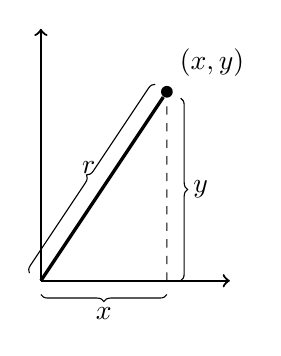
\begin{tikzpicture}[scale=0.8]
        \draw[thick,->] (0,0) coordinate (O) -- (3,0);
        \draw[thick,->] (O) -- (0,4);
        \node[inner sep=1.5pt,fill,circle,label={60:$(x,y)$}] at (2,3) (point) {};
        \draw[very thick] (0,0) -- (point);
        %\draw (1.8,0) -- ++(0,0.2) -- ++(0.2,0);
        \draw[dashed] (2,0) coordinate (pointx) -- (point); 
        \draw[decoration={brace,mirror,raise=5pt},decorate]
        (2,0) -- node[right=6pt] {$y$} (point);
        \draw[decoration={brace,mirror,raise=5pt},decorate]
        (0,0) -- node[below=6pt] {$x$} (2,0); 
        \draw[decoration={brace,raise=5pt},decorate]
        (0,0) -- node[below=6pt] {${}$} (2,3);
        \node [right] at (0.5,1.8) {$r$};
        \end{tikzpicture}
    \end{center} 
\end{frame}



\begin{frame}
        Si $n=3$,  por la aplicación reiterada del teorema de Pitágoras obtenemos que la longitud de $v=(x,y,z)$ es $\sqrt{x^2 + y^2 +z^2}$.\vskip .2cm\pause
    \begin{center}
        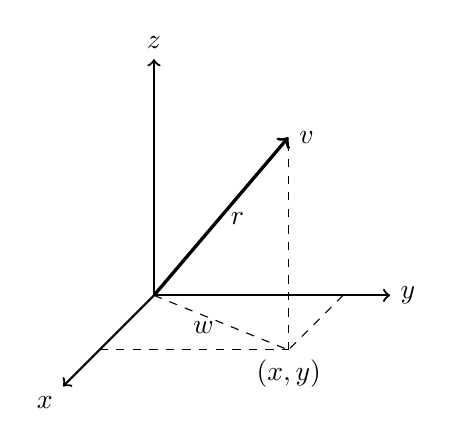
\begin{tikzpicture}[scale=0.6]
        \draw[thick,->] (0,0,0) -- (5,0,0) node[right]{$y$};
        \draw[thick,->] (0,0,0) -- (0,5,0) node[above]{$z$};
        \draw[thick,->] (0,0,0) -- (0,0,5) node[anchor=north east]{$x$};
        \draw[very thick,->] (0,0,0) -- (4,4.5,3) node[anchor=west]{$v$};
        \draw[dashed]  (0,0,0) -- (4,0,3); 
        \draw[dashed]  (0,0,3) -- (4,0,3); 
        \draw[dashed]  (4,0,0) -- (4,0,3); 
        \draw[dashed]  (4,0,3) -- (4,4.5,3); 
        %\draw[decoration={brace,raise=5pt},decorate]
        %(0,0,0) -- node[below=6pt] {${}$} (4,4.5,3);
        \node [right] at (2,2.2,1.5) {$r$};
        \node [right] at (1.2,-0.1,1.5) {$w$};
        \node [below] at (4.2,0.2,3.5) {$(x,y)$};
        \end{tikzpicture}
    \end{center} 
\end{frame}



\begin{frame}
        En  general,  si $v =(x_1,x_2,\ldots,x_n) \in \R^n$ $\Rightarrow$ $    ||v|| = \sqrt{x_1^2+x_2^2+\cdots+x_n^2}$. 
        
        \vskip .4cm\pause
    
    \begin{proposicion}\label{prop-lambda-norma}
        Sea $v \in \R^n$ y $\lambda \in \R$,  entonces
        \begin{equation*}
        ||\lambda v|| = |\lambda|||v||.
        \end{equation*}
    \end{proposicion}
    \begin{proof}\pause
        $||\lambda v||^2 = \la\lambda v, \lambda v \ra$, por \textbf{P3},
        \begin{equation*}
        \la\lambda v, \lambda v \ra = \lambda\la v, \lambda v \ra = \lambda^2\la v, v  \ra.
        \end{equation*}
        Es decir     $||\lambda v||^2 =  \lambda^2 ||v||^2$, por lo tanto, $||\lambda v|| = |\lambda|||v||$.\qed
    \end{proof}
\end{frame}



\begin{frame}{Distancia en $\R^n$}
    \begin{definicion}
        Sea $v,w \in \R^n$, entonce las \textit{distancia}\index{distancia en $\mathbb R^n$} entre $v$ y $w$ es $||v-w||$.
    \end{definicion}
    \vskip .6cm\pause
    \begin{observacion}
        La norma del vector $v-w$ es la longitud del segmento que une $w$ con $v$.        
    \end{observacion}
    
    \begin{center}
        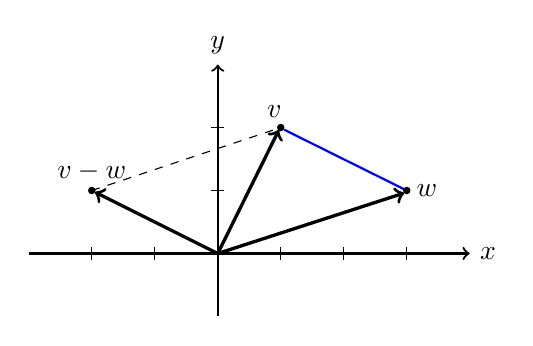
\begin{tikzpicture}[scale=0.8]
        \draw[-, thick,blue] (3,1) -- (1.055,1.965);
        \draw[thick,->] (-3.0,0) -- (4.0,0) node[right] {$x$}; % eje x
        \draw[thick,->] (0,-1) -- (0,3) node[above] {$y$}; % eje y
        \foreach \x in {-2,...,3}
        \draw (\x,3pt) -- (\x,-3pt);
        \foreach \y in {0,...,2}
        \draw (3pt,\y) -- (-3pt,\y) ;
        % vector w
        \draw[fill] (3,1) circle [radius=0.05];
        \node [right] at (3,1) {$w$};
        \draw[very thick, ->] (0,0) -- (2.96,0.96);
        % vector v
        \draw[fill] (1,2) circle [radius=0.05];
        \draw[very thick,->] (0,0) -- (0.97,1.96);
        \node [above] at (0.9,2) {$v$};
        % flecha punteada de w a v
        
        % vector v - w
        \draw[fill] (-2,1) circle [radius=0.05];
        \node [above] at (-2,1) {$v-w$};
        \draw[very thick,->] (0,0) -- (-2*0.975,1*0.975);    
        % punteada de v-w  a v
        \draw[dashed] (-2,1) -- (1,2);    
        \end{tikzpicture}
    \end{center}
\end{frame}


\begin{frame}{Interpretación geométrica del producto escalar}
    Sean   $v_1= (x_1,y_1)$ y $v_2= (x_2,y_2)$ en $\R^2$; veremos a continuación que 
    \begin{equation}\label{eq-cos-theta}
    \langle v_1 , v_2 \rangle = ||v_1||\, ||v_2|| \cos(\theta),
    \end{equation}
    donde  $\theta$ es el ángulo comprendido entre $v_1$ y $v_2$.
    
    \vskip .4cm\pause
    
    Sea $\alpha_1$ el ángulo comprendido  entre $v_1$ y el eje horizontal y $\alpha_2$ el ángulo comprendido  entre $v_2$ y el eje horizontal.  Entonces,
    \begin{equation*}
    v_1 = ||v_1||(\cos (\alpha_1), \sin(\alpha_1) ), \quad v_2 = ||v_2||(\cos (\alpha_2), \sin(\alpha_2) ),
    \end{equation*}\pause
    por lo tanto
    \begin{equation*}
    \langle v_1 , v_2 \rangle =  ||v_1|| \,  ||v_2|| (\cos (\alpha_1)\cos(\alpha_2)+  \sin(\alpha_1)\sin(\alpha_2)). 
    \end{equation*}
\end{frame}



\begin{frame}
    Por otro  lado, por la propiedad de la suma de los cosenos tenemos que 
    \begin{equation*}
    \cos (\alpha_1)\cos(\alpha_2)+  \sin(\alpha_1)\sin(\alpha_2) = \cos(\alpha_1- \alpha_2).
    \end{equation*}
    \vskip .4cm\pause
    Es decir, 
    \begin{equation*}
    \langle v_1,v_2 \rangle =   ||v_1|| \,  ||v_2|| \cos (\alpha_1-\alpha_2), 
    \end{equation*}
    y precisamente, $\theta =  \alpha_1-\alpha_2$ es el ángulo comprendido entre  $v_1$ y $v_2$.
    \vskip .6cm\pause
    Esto se puede  generalizar a  $\R^n$: el ángulo comprendido entre $v_1$ y $v_2$ es 
    \begin{equation*}
    \theta =     \operatorname{arcos}\left(\frac{\langle v_1 , v_2 \rangle}{||v_1|| \,  ||v_2|| }\right).
    \end{equation*}  
\end{frame}


\begin{frame}{Vectores perpendiculares}
    El producto escalar $\langle v , w \rangle$ puede ser  igual a 0 para determinados  vectores,  incluso ambos distintos de 0.  
    \vskip .2cm\pause
    Por ejemplo, si $v = (1,2,3)$ y $w = (2, 1, -\frac43)$,  entonces
    \begin{equation*}
    \langle v , w \rangle = 2 + 2 -4 =0.
    \end{equation*}\pause
    
    \begin{definicion}
        Decimos que dos vectores $v$ y $w$ en $\mathbb R^n$ son  \textit{perpendiculares} u \textit{ortogonales} si  $\langle v , w \rangle=0$. Cuando $v$ y $w$ son ortogonales  denotamos $v \perp w$.
    \end{definicion}
    \vskip .2cm\pause

    
    
\end{frame}


\begin{frame}
    \begin{ejemplo}
        En  $\R^2$ consideremos los vectores
        \begin{equation*}
        v = (3,1),\quad w = (-1, 3),
        \end{equation*}
        representados en la siguiente figura:
        \begin{center}
            \begin{tikzpicture}[scale=1.0]
            \draw[thick,->] (-3.0,0) -- (4.0,0) node[right] {$x$}; % eje x
            \draw[thick,->] (0,-1) -- (0,3) node[above] {$y$}; % eje y
            \foreach \x in {-2,...,3}
            \draw (\x,3pt) -- (\x,-3pt);
            \foreach \y in {0,...,2}
            \draw (3pt,\y) -- (-3pt,\y) ;
            \node [right] at (3,1) {$v$};
            \draw[very thick, ->] (0,0) -- (2.96,0.96);
            \node [above] at (-1,3) {$w$};
            \draw[very thick,->] (0,0) -- (-1*0.975,3*0.975);    
            \end{tikzpicture}
        \end{center}
        
        Luego, vemos que $\langle v , w \rangle = 0$, y por lo tanto $v$  es perpendicular a $w$, lo cual concuerda con nuestra intuición. 
    \end{ejemplo}
\end{frame}


\begin{frame}
        
    Es claro que esta definición algebraica de perpendicularidad está de acuerdo con la interpretación geométrica del producto escalar:
    
    \vskip .2cm
    \begin{center}
        $v$ y $w$ perpendiculares (geométricamente)
        \vskip .2cm \pause
        $\Downarrow$ 
        \vskip .2cm    
        el ángulo comprendido entre $v$ y $w$ es $\theta = 90^\circ$
        \vskip .2cm\pause
            $\Downarrow$ 
        \vskip .2cm    
        $\cos(\theta) = 0$
        \vskip .2cm\pause 
        $\Downarrow$ 
        \vskip .2cm    
        $\langle v , w \rangle = ||v||\, |w|| \cos(\theta) = 0$.
    \end{center}
    
    

\end{frame}



\end{document}

